\section{Experimento Laboratorial}

Nesta etapa, o circuito proposto foi montado fisicamente em bancada utilizando
componentes reais disponíveis no laboratório.

\begin{figure}[H]
  \centering
  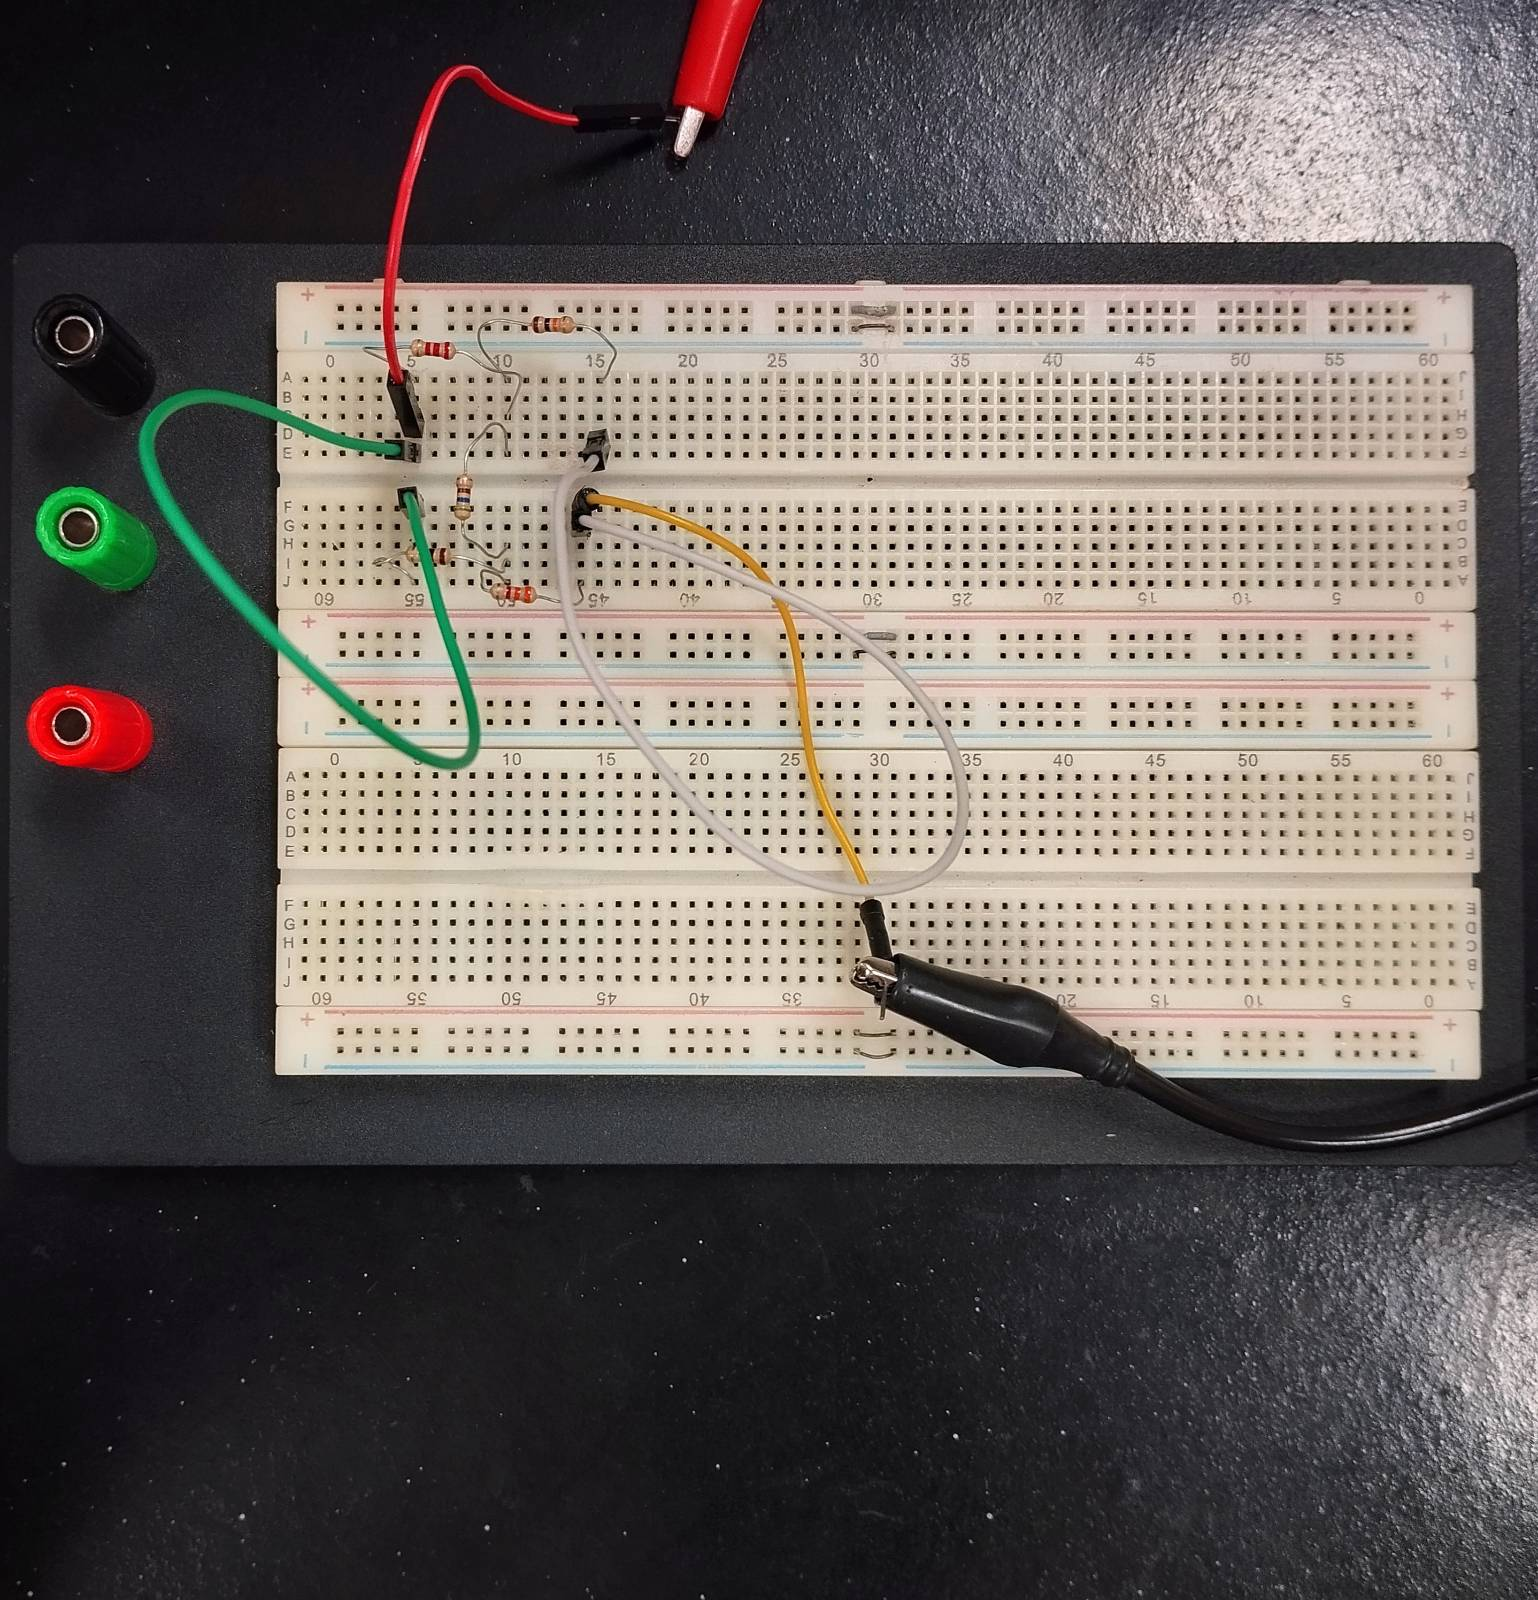
\includegraphics[width=0.5\linewidth]{fig/lab1realcircuit.jpeg}
  \caption{Circuito montado em laboratório}
  \label{fig:real-circuit}
\end{figure}

\begin{figure}[H]
  \centering
  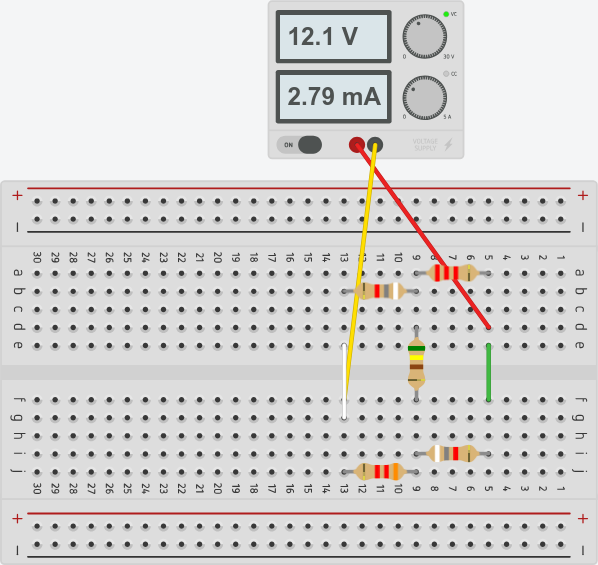
\includegraphics[width=0.5\linewidth]{fig/lab1tinkercad.png}
  \caption{Circuito recreado no Tinkercad para melhor visualização}
  \label{fig:tinkercad}
\end{figure}

Ao realizar medições com multímetros de bancada, foram observadas variações nos
valores nominais dos componentes, como apresentado a seguir:

\begin{itemize}
  \item Fonte: \(V = \SI{12.01}{\volt} \neq \SI{12}{\volt}\)
  \item \(R_1 = \SI{2.15}{k\ohm} \neq \SI{2.2}{k\ohm}\)
  \item \(R_2 = \SI{9.78}{k\ohm} \neq \SI{10}{k\ohm}\)
  \item \(R_3 = \SI{540}{\ohm} \neq \SI{560}{\ohm}\)
  \item \(R_4 = \SI{9.83}{k\ohm} \neq \SI{10}{k\ohm}\)
  \item \(R_5 = \SI{3.20}{k\ohm} \neq \SI{3.3}{k\ohm}\)
\end{itemize}

Estas discrepâncias entre os valores reais e ideais são esperadas em contextos
experimentais. Elas resultam de fatores como:

\begin{itemize}
  \item Tolerância dos componentes, geralmente indicada no corpo dos resistores
  (por exemplo, 5\% ou 1\%);
  \item Variações na tensão de alimentação, especialmente se a fonte não for
  regulada com precisão;
  \item Influências ambientais como temperatura e umidade, que podem afetar
  levemente a resistência elétrica.
\end{itemize}

As tensões e correntes em cada resistor e na fonte foram medidas em laboratório e serão apresentadas na seção de Resultados (\ref{sec:resultados}).